\documentclass[11pt]{article}
\usepackage{amsmath}
\usepackage{amssymb}
\usepackage{amsthm}
\usepackage{caption}
\usepackage{cleveref}
\usepackage{enumitem}
\usepackage{graphicx}
\usepackage[totalwidth=480pt, totalheight=680pt]{geometry}
\usepackage{mathrsfs}
\usepackage{tikz}
\usetikzlibrary{calc}
\usepackage{xcolor}
\usepackage[round]{natbib}
\definecolor{mid_green}{HTML}{99d8c9}

\captionsetup{width=0.8\textwidth}
\DeclareMathOperator*{\argmax}{arg\,max}
\newtheorem{corollary}{Corollary}
\newtheorem{definition}{Definition}
\newtheorem{lemma}[corollary]{Lemma}
\newtheorem{theorem}[corollary]{Theorem}
\setlength{\tabcolsep}{1em}
\setlist{listparindent=\parindent, parsep=0pt}

\newcommand{\EE}{\mathbb{E}}
\newcommand{\PP}{\mathbb{P}}
\newcommand{\RR}{\mathbb{R}}
\newcommand{\ZZ}{\mathbb{Z}}

% Commands for inline commenting that shows up on pdf
\newcommand{\WFcomment}[1]{{\color{red}{(WF: \bf \sc #1) }}}
\newcommand{\KHcomment}[1]{{\color{green!60!black}{(KH: \bf \sc #1) }}}

\begin{document}

\title{Rank Verification for Exponential Families}
\author{Kenneth Hung \and William Fithian}
\date{\today}
\maketitle

\begin{abstract}
Many statistical experiments involve comparing multiple population groups. For example, a public opinion poll may ask which of several political candidates commands the most support, or a clinical trial may compare patient outcomes to determine the best of several treatment conditions. This article concerns the problem of {\em rank verification} --- post hoc tests of whether the ordering discovered in the data is in fact statistically significant. For exponential family models, we show under mild conditions that an unadjusted two-tailed pairwise test comparing the ``winning'' population to the ``runner-up'' is a valid test of whether the winner is truly the best. We also propose comparably simple procedures to give lower confidence bounds on the gap between the winning population and the others, and to verify ranks beyond the first.
\end{abstract}

\section{Introduction}
\label{sec:intro}

\subsection{Motivating Example: Iowa Republican Caucus Poll}
\label{sec:iowa}

\Cref{tbl:poll} shows the result of a Quinnipiac University poll asking 890 Iowa Republicans their preferred candidate for the Republican presidential nomination \citep{quinnipiac}. Donald Trump led with $31\%$ of the vote, Ted Cruz came second with $24\%$, Marco Rubio third with $17\%$, and ten other candidates including ``Don't know'' trailed behind. 

\begin{table}[htbp]
\begin{center}
\begin{tabular}{c c c c}
	\hline
	Rank & Candidate & Result & Votes \\
	\hline
	$1$ * & Trump & $31\%$ & $276$ \\
	$2$ * & Cruz & $24\%$ & $214$ \\
	$3$ * & Rubio & $17\%$ & $151$ \\
	$4$ * & Carson & $8\%$ & $71$ \\
	$5$ & Paul & $4\%$ & $36$ \\
	$6$ & Bush & $4\%$ & $36$ \\
	$7$ & Huckabee & $3\%$ & $27$ \\
	$\vdots$ & $\vdots$ & $\vdots $ & $\vdots$ \\
	\hline
\end{tabular}
\end{center}
\caption{Results from a February 1, 2016 Quinnipiac University poll of $890$ Iowa Republicans. To compute the last column (Votes), we make the simplifying assumption that the reported percentages in the third column (Result) correspond to raw vote shares among survey respondents. The asterisks indicate that the rank is verified at $0.05$-level through a step-down procedure.}
\label{tbl:poll}
\end{table}

Seeing that Trump leads this poll, several salient questions may occur to us: Is Trump really winning, and if so by how much? And analogously, is Cruz really in second, is Rubio really in third, and so on? Note that there is implicitly a problem of multiple comparisons here, because if Cruz had led the poll instead, we would be asking a different set of questions. Indeed, the selection issue appears especially pernicious due to the so-called ``winner's curse'': given that Trump leads the poll, it more likely than not overestimates his support.

Nevertheless, if we blithely ignore the selection issue, we might carry out the following analyses to answer the questions we posed before at significance level $\alpha = 0.05$. We assume for simplicity that the poll represents a simple random sample of Iowa Republicans; i.e., that the data are a multinomial sample of size $890$ and underlying probabilities $\left(\pi_{\text{Trump}}, \pi_{\text{Cruz}}, \ldots\right)$.\footnote{The reality is a bit more complicated: before releasing the data, Quinnipiac has processed it to make the reported result more representative of likely caucus-goers.}

\begin{enumerate}
\item {\em Is Trump really winning?} If Trump and Cruz were in fact tied, then Trump's share of their combined 490 votes would be distributed as $\text{Binom}\left(490, 0.5\right)$. Because the (two-tailed) $p$-value for this pairwise test is $p = 0.006$, we reject the null and conclude that Trump is really winning.

\item {\em By how much?} Using an exact $95\%$ interval for the same binomial model, we conclude Trump has at least $7.5\%$ more support than Cruz (i.e., $\pi_{\text{Trump}} \ge 1.075 \,\pi_{\text{Cruz}}$) and also leads the other candidates by at least as much.

\item {\em Is Cruz in second, Rubio in third, etc.?} We can next compare Cruz to Rubio just as we compared Trump to Cruz (again rejecting because $214$ is significantly more than half of 365), then Rubio to Carson, and so on, continuing until we fail to reject. The first four comparisons are all significant at level $0.05$, but Paul and Bush are tied so we stop.
\end{enumerate}

Surprisingly, all of the three procedures described above are statistically valid despite ignoring the implicit multiple-comparisons issue. The remainder of this article is dedicated to justifying these procedures for the multinomial family and analogous procedures in other settings.

\subsection{Generic Problem Setting and Main Result}
\label{sec:probset}

Generically, we will consider data drawn from an exponential family model with density
\begin{equation}
X \sim \exp\left(\theta'x - \psi\left(\theta\right)\right) g\left(x\right),
\label{eqn:expfam}
\end{equation}
with respect to either the Lebesgue measure on $\RR^n$ or counting measure on $\ZZ^n$. We assume further that $g\left(x\right)$ is symmetric with respect to permutation, and Schur concave, a mild technical condition defined in \Cref{sec:maj}. In addition to the multinomial family, model~\eqref{eqn:expfam} also encompasses settings such as comparing independent binomial treatment outcomes in a clinical trial, competing sports teams under a Bradley--Terry model, entries of a Dirichlet distribution, and many more; see \Cref{sec:examples} for these and other examples.

We will generically use the term {\em population} to refer to the treatment group, sports team, political candidate, etc. represented by a given random variable $X_j$. As we will see, $\theta_j \ge \theta_k$ if and only if $X_j$ is stochastically larger than $X_k$; thus, there is a well-defined stochastic ordering of the populations that matches the ordering of the entries of $\theta$. We will refer to the population with maximal $\theta_j$ as the {\em best}, the one with maximal $X_j$ as the {\em winner}, and the one with maximal $X_j$ other than the winner as the {\em runner-up}. Following the convention in the ranking and selection literature, we assume that if there are multiple largest $\theta_j$, then one is arbitrarily marked as the best. Note that in cases where it is more interesting to ask which is the smallest population (for example, if $X_j$ is the number of patients on treatment $j$ who suffer a heart attack during a trial) we can change the variables to $-X$ and the parameters to $\theta$. 

Write the order statistics of $X$ as
$$X_{[1]} \ge X_{[2]} \ge \cdots \ge X_{[n]},$$
where $[j]$ will denote the random index for the $j$-th order statistic. Define $\theta_{[j]}$ as the entry of $\theta$ corresponding to the $j$-th order statistic of $X$ (so $\theta_{[1]}$ might {\em not} equal $\max_j \theta_j$, for example). We assume any ties between entries of $X$ are broken randomly.

In each of the above examples, there is a natural exact test we could apply to test $\theta_j=\theta_k$ for any two {\em fixed} populations $j$ and $k$. In the multinomial case, we would apply the conditional binomial test based on the combined total $X_j+X_k$ as discussed in the previous section. For the case of independent binomials we would apply Fisher's exact test, again conditioning on $X_j+X_k$. These are both examples of a generic UMPU pairwise test in which we condition on the other $n-2$ indices (notated $X_{\setminus \{j,k\}}$) and $X_j+X_k$, and reject the null if $X_j$ is outside the $\alpha/2$ and $1-\alpha/2$ quantiles of the conditional law $\mathcal{L}_{\theta_j=\theta_k}(X_j \mid X_j+X_k, X_{\setminus\{j,k\}})$, which crucially does not depend on the value of $\theta_j$ or $\theta_k$. We call this test the (two-tailed) {\em unadjusted pairwise test} since it makes no explicit adjustment for selection. Similarly, inverting this test for all values of $\theta_j-\theta_k$ yields an {\em unadjusted pairwise confidence interval}.\footnote{To avoid trivialities in the discrete case, we assume these procedures are appropriately randomized at the rejection thresholds to give exact level-$\alpha$ control.}

Generalizing the procedures described in \Cref{sec:iowa} we obtain the following:
\begin{enumerate}
\item {\em Is the winner really the best?} Carry out the unadjusted pairwise test comparing the winner to the runner-up. If the test rejects at level $\alpha$, conclude that the winner is really the best.
\item {\em By how much?} Construct the unadjusted pairwise confidence interval comparing the winner to the runner-up, and report the lower confidence bound obtained for $\theta_{[1]}-\theta_{[2]}$ if it is nonnegative, report $-\infty$ otherwise.
\item {\em Is the runner-up really the second best, etc.?} Continue by comparing the runner-up to the second-runner-up, again using the unadjusted pairwise test, and so on down the list comparing adjacent values. Stop the first time the test accepts.
\end{enumerate}
Procedure $2$ is modified above due to some technicalities. If reporting $-\infty$ seems extreme, we included a gentler modification in this paper as well.

We now state our main theorem: under a mild technical assumption, Procedures 1--3 described above are statistically valid, even accounting for the selection.
\begin{theorem}
Assume the model~\eqref{eqn:expfam} holds and $g\left(x\right)$ is a Schur-concave function. Then:
\begin{enumerate}
\item Procedure 1 has level $\alpha$ conditional on the best population not winning (otherwise an error is impossible).
\item Procedure 2 gives a conservative $1-\alpha$ lower confidence bound for $\theta_{[1]} - \max_{j \ne [1]} \theta_{j}$.
\item Procedure 3 is a conservative step-down procedure with familywise error rate (FWER) no larger than $\alpha$.
\end{enumerate}
\label{thm:main}
\end{theorem}

We define Schur-concavity and discuss its properties in \Cref{sec:maj}. Because any log-concave and symmetric function is Schur-concave, \Cref{thm:main} applies to all of the cases discussed above. The proof relies on the conditional selective-inference framework of \citet{Fithian:2014ws} combined with classical multiple-testing methods, as well as some properties of majorization and Schur-concavity.

Note that these procedures make an implicit adjustment for selection because they use two-tailed unadjusted tests. If we instead based our tests on an independent realization $X^*$, then, for example, Procedure 1 could use a right-tailed version of the unadjusted pairwise test. In the case $n = 2$, Procedure 1 amounts to a simple two-tailed test of the null hypothesis $\theta_1 = \theta_2$, and it is intuitively clear that a one-tailed test would be anti-conservative. More surprising is that, no matter how large $n$ is, Procedures 1--3 require no further adjustment beyond what is required when $n = 2$. 

\subsection{Related work}

Previous works construct tests comparing parameters in various families of distributions, by comparing just the winner and the runner-up. \citet{Gutmann:1987fk} tackles the question where the observations are from a location family, and the location parameters are compared. In which case, the difference of the winner and the runner-up has to pass a predetermined threshold. In contrast, a related paper by \citet{Karnnan:2009iv} discusses a scale family, comparing the scale parameters instead. Specifically, to test for the smallest variance across multiple populations, it is sufficient to test the ratio of the smallest to the second-smallest variances. \citet{Bofinger:1991hv} gives a location-scale family generated by translating an exponential distribution as well. Similarly, test the difference between the winner and the runner-up is enough. A follow-up paper by \citet{Maymin:1992fz} gave an analogous result for location-scale families, yet still under the constraints of independence as well.

However, as location-scale families have limited overlap with exponential families, the counterpart question for exponential families remains unaddressed. Location-scale families assumes independence between observations, while this is not required in exponential families. For instance, in the vicinity of the polling problem above, \citet{Nettleton:2009ht} provides an asymptotic test for multinomial distribution, imposing the selection by considering intersection-union tests. \citet{Ng:2007cn} also analyzes the multinomial case for an exact test, but with an additional restriction that maximum observation is a known constant $M$. In terms of the polling problem above, we poll until one candidate hits a goal $M$. While in either papers the observations $X$ are not independent, it still suffices to test the difference between the winner and the runner-up.

One final result that our particular interest in the subset selection problem \citep{Gupta:1967wg}. It can indeed be used to solve the multinomial case. They select a subset that contains the largest, or ``tagged'', parameter with probability $1-\alpha$. Confirming the largest parameter is thus equivalent to asserting the selected subset has size $1$. \Cref{sec:subsetsel} includes a comparison of our proposed test and their test.

\subsection{Outline}
\Cref{sec:maj} gives a formal definition of Schur-concavity, as well as common examples satisfying this condition. \Cref{sec:winnerbest} proves that an unadjusted pairwise test comparing the winner to the runner-up is valid, and demonstrates the power of this test. \Cref{sec:confbound,sec:stepdown} justify Procedures 2 and 3. We conclude by examining a published study with our methods in \Cref{sec:disc}.

\section{Majorization and Schur-concavity}
\label{sec:maj}

We start by reviewing the notion of {\em majorization}, defined on both $\RR^n$ and $\ZZ^n$.

\begin{definition}
For two vectors $a$ and $b$ in $\RR^n$ (or $\ZZ^n$), suppose sorting the two vectors in descending order gives
$a_{\left(1\right)} \ge \cdots \ge a_{\left(n\right)}$ and $b_{\left(1\right)} \ge \cdots \ge b_{\left(n\right)}$. We say that $a \succeq b$ ($a$ majorizes $b$) if for $1 \le i < n$,
\begin{align*}
a_{\left(1\right)} + \cdots + a_{\left(i\right)} & \ge b_{\left(1\right)} + \cdots + b_{\left(i\right)} \\
a_{\left(1\right)} + \cdots + a_{\left(n\right)} & = b_{\left(1\right)} + \cdots + b_{\left(n\right)}
\end{align*}
This forms a partial order in $\RR^n$ (or $\ZZ^n$).
\end{definition}

Intuitively, majorization is a partial order that monitors the evenness of a vector: the more even a vector is, the ``smaller'' it is. There are two properties of majorization that we will use in the proofs.

\begin{lemma}
\begin{enumerate}
\item Suppose $\left(x_1, x_2, x_3, \ldots\right)$ and $\left(x_1, x_2', x_3' \ldots\right)$ are two vectors in $\RR^n$. Then
$$\left(x_1, x_2, x_3, \ldots\right) \succeq \left(x_1, x_2', x_3', \ldots\right) \text{ if and only if } \left(x_2, x_3, \ldots\right) \succeq \left(x_2', x_3', \ldots\right).$$
\item (Principle of transfer) If $x_1 > x_2$ and $t \ge 0$, then
$$\left(x_1 + t, x_2, x_3, \ldots\right) \succeq \left(x_1, x_2 + t, x_3\right).$$
If the $t \le 0$, the majorization is reversed.
\end{enumerate}
\label{lma:twoprop}
\end{lemma}

\begin{proof}
\begin{enumerate}
\item The property follows from an equivalent formulation of majorization listed in \citet{Marshall:2010hb}, where $x \succeq y$ if and only if
$$\sum_{j=1}^n x_n = \sum_{j=1}^n y_n ~~~~ \text{ and } ~~~~ \sum_{j=1}^n \left(x_j - a\right)_+ \ge \sum_{j=1}^n \left(y_j - a\right)_+ \text{ for all } a \in \RR.$$

\item Proved in \citet{Marshall:2010hb}. \qedhere
\end{enumerate}
\end{proof}

\begin{definition}
A function $g$ is Schur-concave if $x \succeq y$ implies $g\left(x\right) \le g\left(y\right)$.
\end{definition}

A Schur-concave function is symmetric by default since $a \succeq b$ and $b \succeq a$ if and only if $b$ is a permutation of the coordinates of $a$. Conversely a symmetric and log-concave function is Schur-concave \citep{Marshall:2010hb}, thus many common exponential family distributions lie in this class. Schur-concave functions indeed appear a lot, \Cref{sec:examples} includes both continuous and discrete examples.

\Cref{thm:main} requires that $g\left(x\right)$ in model~\eqref{eqn:expfam} to be Schur-concave. It was stated in the ensuing discussion that this condition is mild, and that the examples are abundant. To name a few:

\subsection{Examples}
\label{sec:examples}

\begin{enumerate}
\item Independent binomial treatment outcome in a clinical trial. If each of the $n$ different treatments are applied $m$ patients independently, the number of positive outcomes $X_j$ for treatment $j$ can be modeled by $\text{Binomial}\left(m, p_j\right)$. The best treatment would be the treatment with the highest success probability $p_j$. The joint distribution of $X$ is given by
$$p\left(x\right) \propto \exp\left(x' \left(\log p\right)\right) \frac{1}{x_1! \left(m-x_1\right)! \cdots x_n! \left(m-p_x\right)!}$$
The carrier measure above is Schur-concave.

\item Competing sports under Bradley--Terry model. Suppose $n$ players held a round robin tournaments with the Bradley--Terry model, where player $j$ has a score $\theta_j$, and the probability of player $j$ winning against player $k$ is
$$\frac{e^{\theta_j - \theta_k}}{1 + e^{\theta_j - \theta_k}} = \frac{e^{\left(\theta_j - \theta_k\right) / 2}}{e^{\left(\theta_j - \theta_k\right) / 2} + e^{\left(\theta_k - \theta_j\right) / 2}}.$$

Let $Y_{jk}$ be an indicator for the match between player $j$ and $k$, where we take $Y_{jk} = 1$ if $j$ beats $k$ and $Y_{jk} = 0$ if $k$ beats $j$. For symmetry, we will also adopt the convention that $Y_{jk} + Y_{kj} = 1$. Thus the joint distribution of $\left(Y_{jk}\right)_{j, k}$ is
$$p\left(\left(y_{jk}\right)_{j, k}\right) \propto \exp\left(\sum_j 2\theta_j \sum_{k \ne j} y_{jk}\right)  = \exp\left(2\theta' x\right),$$
where $x_j = \sum_{k \ne j} y_{jk}$. In other words, $x_j$ is the number of wins by player $j$.

If the individual results are masked and we only know about the net wins, then
$$p\left(x\right) \propto \exp\left(2\theta' x\right) g\left(x\right),$$
where $g\left(x\right)$ is a function that count number of possible tournament results giving the net win vector $x$. A bijection proof shows that $x$ is indeed Schur-concave.

\item Comparing the variances of different normal populations. Suppose there are $n$ normal populations with laws $N\left(\mu_j, \sigma_j^2\right)$ and $m$ independent observations from each of them. The sample variance for population $j$ can be denoted as $r_j$. By Cochran's theorem, $\left(m-1\right) r_j \sim \sigma_j^2 \chi_{m-1}^2$, and thus the joint distribution of $r$ is
\begin{align*}
r & \sim \prod_{j=1}^n \left(\frac{\left(m-1\right) r_j}{\sigma_j^2}\right)^{\left(m-3\right) / 2} e^{-\left(m-1\right) r_j / 2 \sigma_j^2} 1_{\left\{r_j > 0 \right\}} \\
& \propto \exp\left(-\frac{m-1}{2 \sigma_1^2} r_1 - \cdots - \frac{m-1}{2 \sigma_n^2} r_n\right) \prod_{j=1}^n r_j^{\left(m-3\right) / 2} 1_{\left\{r > 0\right\}}.
\end{align*}
The carrier measure is $\prod_{j=1}^n r_j^{\left(m-3\right) / 2} 1_{\left\{r > 0\right\}}$, which is Schur-concave.
\end{enumerate}

\section{Is the Winner Really the Best?}
\label{sec:winnerbest}

The following lemma should clarify the key idea in the proof of the theorem.

\begin{lemma}
If $p_j$ are valid $p$-values for testing null hypothesis $H_{0j}$, then $p_* = \max_j p_j$ is a valid $p$-value for the union null hypothesis $H_0 = \bigcup_j H_{0j}$. If all the $p$-values are exact, then $p_*$ is also an exact $p$-value.
\label{lma:union}
\end{lemma}

\begin{proof}
Since $p_j$ are all valid $p$-values,
$$\PP_{H_{0j}}\left(p_j < \alpha\right) \le \alpha.$$
S for the union null hypothesis
$$\PP_{H_0}\left(p_* < \alpha\right) = \max_j \PP_{H_{0j}}\left(p_* < \alpha\right) \le \max_j \PP_{H_{0j}}\left(p_j < \alpha\right) \le \alpha.$$
And thus $p_*$ is a valid $p$-value for the union null hypothesis. Now if $p_j$ are all exact, then equality holds above and $p_*$ is exact as well.
\end{proof}

We are now ready to prove our result for Procedure 1.

\begin{theorem}
Assume the model~\eqref{eqn:expfam} holds and $g\left(x\right)$ is a Schur-concave function. Procedure 1 (the unadjusted pairwise test) has level $\alpha$ conditional on the best population not winning.
\label{thm:seltest}
\end{theorem}

\begin{proof}
Without loss of generality, otherwise by relabeling, we consider only the case where the winner is $1$ and the runner-up is $2$, etc., i.e.\ $X_1 \ge \cdots \ge X_n$. In this case, we will test the null hypothesis $H_{01}: \theta_1 \le \max_{j > 1} \theta_j$, which is the union of the null hypotheses $H_{01j}: \theta_1 \le \theta_j$ for $j > 1$. For each of these we can construct an exact $p$-value $p_{1j}$. Hence by \Cref{lma:union}, a test based on $p_{1*} = \max_j p_{1j}$ would be exact for $H_{01}$. Procedure 1 will perform an unadjusted pairwise test comparing $X_1$ to $X_2$. Hence it is sufficient to show that $p_{12} = p_{1*}$ and that the test based on $p_{12}$ coincides with the unadjusted pairwise test.

Following the framework in \citet{Fithian:2014ws}, we consider the selection event where the winner is $1$: $$A_1 = \left\{X_1 \ge \max_{j > 1} X_j\right\}.$$
For convenience, we let
$$D_{jk} = \frac{X_j - X_k}{2} ~~~~ \text{ and } ~~~~ M_{jk} = \frac{X_j + X_k}{2}.$$

We start by re-parametrizing to replace $X_1$ and $X_j$ with $D_{1j}$ and $M_{1j}$ and consider
\begin{equation}
\mathcal{L}_{\theta_1 - \theta_j = 0} \left(D_{1j} \middle| M_{1j}, X_{\setminus\left\{1, j\right\}}, A_1\right), \text{ where } A_1 = \left\{D_{1j} \ge \max_{k \ne 1, j} X_k - M_{1j}\right\} \cap \left\{D_{1j} \ge 0\right\}.
\label{eqn:condlaw}
\end{equation}
The conditional law in \Cref{eqn:condlaw}, in particular, is a truncated distribution
\begin{align*}
D_{1j} & \sim \exp\left(\left(\theta_1 - \theta_j\right) D_{1j} + \theta_2 X_2 + \cdots + \left(\theta_1 + \theta_j\right) M_{1j} + \cdots + \theta_n X_n \right) \\
& ~~~~~~~~ g\left(M_{ij} + D_{ij}, X_2, \ldots, M_{ij} - D_{ij}, \ldots X_n\right) 1_{A_1} \\
& \sim g\left(M_{ij} + D_{ij}, X_2, \ldots, M_{ij} - D_{ij}, \ldots X_n\right) 1_{A_1}.
\end{align*}

The $p$-value for $H_{01j}$ is thus
\begin{equation}
p_{1j} = \frac{\int_{D_{1j}}^\infty g\left(M_{1j} + z, X_2, \ldots, M_{1j} - z, \ldots, X_n\right) \,dz}{\int_{\max\left\{X_2 - M_{1j}, 0\right\}}^\infty g\left(M_{1j} + z, X_2, \ldots, M_{1j} - z, \ldots, X_n\right) \,dz}.
\label{eqn:p1j}
\end{equation}

By construction, $p_{1j}$ satisfies
$$\PP_{H_{01j}}\left(p_{1j} < \alpha \middle| M_{1j}, X_{\setminus\left\{1, j\right\}}, A_1\right) = \alpha.$$
Taking expectation on both sides gives
$$\PP_{H_{01j}}\left(p_{1j} < \alpha \middle| A_1\right) = \alpha.$$
Therefore these $p_{1j}$ are indeed valid exact $p$-values.

Without loss of generality, it is sufficient to show that $p_{12} \ge p_{13}$. In the computation of either $p$-values, $X_4, \ldots, X_n$ are all conditioned on. The first point in \Cref{lma:twoprop} says that we may assume $n = 3$ without affecting the Schur-concavity of $g$. This allows us to clean up our notation and
\begin{align*}
p_{12} & = \frac{\int_{D_{12}}^\infty g\left(M_{12} + z, M_{12} - z, X_3\right) \,dz}{\int_0^\infty g\left(M_{12} + z, M_{12} - z, X_3\right) \,dz} \\
p_{13} & = \frac{\int_{D_{13}}^\infty g\left(M_{13} + z, X_2, M_{13} - z\right) \,dz}{\int_{\max\left\{X_2 - M_{13}, 0\right\}}^\infty g\left(M_{13} + z, X_2, M_{13} - z\right) \,dz}
\end{align*}

Suppose $X_2 < M_{13}$, then we can re-parametrize the integrals above to give
\begin{align*}
p_{12} & = \frac{\int_0^\infty g\left(X_1 + z, X_2 - z, X_3\right) \,dz}{\int_0^\infty g\left(M_{12} + z, M_{12} - z, X_3\right) \,dz} \\
& = \frac{\int_0^\infty g\left(X_1 + z, X_2 - z, X_3\right) \,dz}{\int_{-D_{12}}^\infty g\left(X_1 + z, X_2 - z, X_3\right) \,dz} \\
p_{13} & = \frac{\int_0^\infty g\left(X_1 + z, X_2, X_3 - z\right) \,dz}{\int_0^\infty g\left(M_{13} + z, X_2, M_{13} - z\right) \,dz} \\
& = \frac{\int_0^\infty g\left(X_1 + z, X_2, X_3 - z\right) \,dz}{\int_{-D_{13}}^\infty g\left(X_1 + z, X_2, X_3 - z\right) \,dz}
\end{align*}
To help see the re-parametrization, each of these integrals can be thought of in terms integrals along segments and rays. For example $p_{12}$ can be represented in terms integrals $A$ and $B$ in \Cref{fig:p-value}. Specifically,
$$p_{12} = \frac{B}{A + B}$$

\begin{figure}[htbp]
\begin{center}
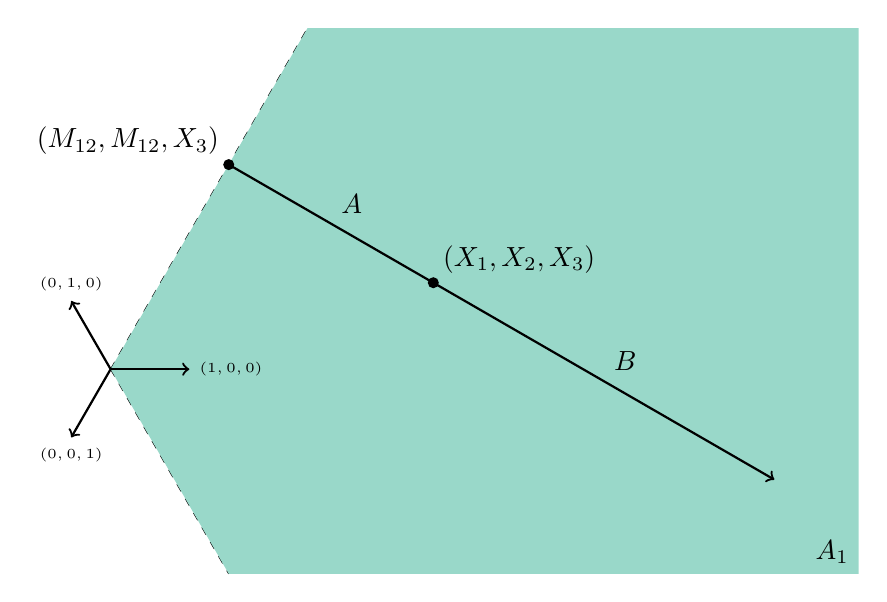
\begin{tikzpicture}
	\coordinate (C1) at (60:5);
	\coordinate (C2) at (300:3);
	\coordinate (A) at (60:3);
	\coordinate (B) at ($(A) + (330:3)$);
	\draw[dashed] (0, 0) -- (C1);
	\draw[dashed] (0, 0) -- (C2);
	\fill[mid_green] (0, 0) -- (C1) -- ($(C1) + (7, 0)$) -- ($(C2) + (8, 0)$) -- (C2) -- cycle;
	\node[above left] at ($(C2) + (8, 0)$) {$A_1$};
	\draw[thick] (A) -- (B) node[midway, above right] {$A$};
	\draw[thick, ->] (B) -- ++(330:5) node[midway, above right] {$B$};
	\fill (A) circle(2pt) node[above left] {$\left(M_{12}, M_{12}, X_3\right)$};
	\fill (B) circle(2pt) node[above right] {$\left(X_1, X_2, X_3\right)$};
	\draw[thick, ->] (0, 0) -- (1, 0) node[right] {\tiny $\left(1, 0, 0\right)$};
	\draw[thick, ->] (0, 0) -- (120:1) node[above] {\tiny $\left(0, 1, 0\right)$};
	\draw[thick, ->] (0, 0) -- (240:1) node[below] {\tiny $\left(0, 0, 1\right)$};
\end{tikzpicture}
\end{center}
\caption{The $p$-value $p_{12}$ can be written in terms of integral $A$ along the segment and $B$ along the ray. The diagram is drawn a level set of $x_1 + x_2 + x_3$. The green region represents the selection event $A_1$.}
\label{fig:p-value}
\end{figure}

\Cref{fig:compare_rays} has both the $p$-values shown on the same diagram. Proving $p_{12} \ge p_{13}$ is the same as proving
$$\frac{B}{A+B} \ge \frac{D}{C+D} ~~~~ \Longleftrightarrow ~~~~ \frac{B}{A} \ge \frac{D}{C}.$$
We will prove so by extending $A$ to include $\tilde{A}$ on the diagram. We denote the sum $A + \tilde{A}$ as $A'$. Formally,
\begin{equation}
A' = \int_{-D_{13}}^0 g\left(X_1 + z, X_2 - z, X_3\right) \,dz \ge \int_{-D_{12}}^0 g\left(X_1 + z, X_2 - z, X_3\right) \,dz = A.
\label{eqn:int_extension}
\end{equation}
It is thus sufficient to show that $B \ge D$ and $C \ge A'$.

\begin{figure}[htbp]
\begin{center}
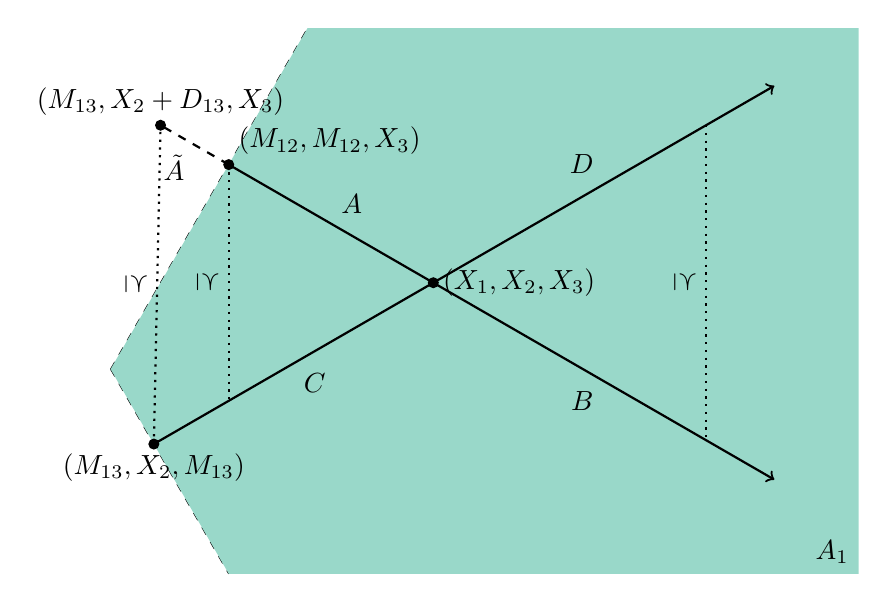
\begin{tikzpicture}
	\coordinate (C1) at (60:5);
	\coordinate (C2) at (300:3);
	\coordinate (A) at (60:3);
	\coordinate (B) at ($(A) + (330:3)$);
	\coordinate (C) at ($(0, 0)!(B)!(C2)$);
	\coordinate (D) at ($(A) + (150:1)$);
	\draw[dashed] (0, 0) -- (C1);
	\draw[dashed] (0, 0) -- (C2);
	\fill[mid_green] (0, 0) -- (C1) -- ($(C1) + (7, 0)$) -- ($(C2) + (8, 0)$) -- (C2) -- cycle;
	\node[above left] at ($(C2) + (8, 0)$) {$A_1$};
	\draw[thick] (A) -- (B) node[midway, above right] {$A$};
	\draw[thick, ->] (B) -- ++(330:5) node[midway, below left] {$B$};
	\fill (A) circle(2pt) node[above right] {$\left(M_{12}, M_{12}, X_3\right)$};
	\fill (B) circle(2pt) node[right] {$\left(X_1, X_2, X_3\right)$};
	\draw[thick] (C) -- (B) node[midway, below right] {$C$};
	\node[below] at (C) {$\left(M_{13}, X_2, M_{13}\right)$};
	\draw[thick, ->] (B) -- ++(30:5) node[midway, above left] {$D$};
	\fill ($(0, 0)!(B)!(C2)$) circle(2pt);
	\draw[thick, dashed] (A) -- (D) node[midway, below left] {$\tilde{A}$};
	\fill (D) circle(2pt) node[above] {$\left(M_{13}, X_2 + D_{13}, X_3\right)$};
	\draw[thick, dotted] (C) -- (D) node[midway, below, rotate=-90] {$\succeq$};
	\draw[thick, dotted] (A) -- ++(0, -3) node[midway, below, rotate=-90] {$\succeq$};
	\draw[thick, dotted] ($(B) + (30:4)$) -- ($(B) + (330:4)$) node[midway, below, rotate=-90] {$\succeq$};
\end{tikzpicture}
\end{center}
\caption{The $p$-value $p_{12}$ can be written in terms of integral $A$ along the segment and $B$ along the ray; and $p_{13}$ in terms of $C$ and $D$. $A'$ would refer to the sum of $A$ with the dashed line portion labeled as $\tilde{A}$, formally explained in \Cref{eqn:int_extension}. The majorization relation is indicated by the dotted line.}
\label{fig:compare_rays}
\end{figure}

Indeed from the second point in \Cref{lma:twoprop} we have
$$\left(X_1 + z, X_2 - z, X_3\right) \succeq \left(X_1 + z, X_2, X_3 - z\right)$$
for $z \le 0$ and the majorization reversed for $z \ge 0$. This majorization relation is indicated as the dotted line in \Cref{fig:compare_rays}. So Schur-concavity shows that
$$g\left(X_1 + z, X_2 - z, X_3\right) \le g\left(X_1 + z, X_2, X_3 - z\right)$$
for $z \le 0$, and the inequality reversed for $z \ge 0$. Taking integrals on both sides yields the desired inequality.

For the alternative case where $X_2 \ge M_{13}$, the segment $C$ will reach the line $x_1 = x_2$ first before it reach $x_1 = x_3$, ending at $\left(X_2, X_2, X_1 - X_2 + X_3\right)$ instead. But we can still extend $A$ by $\tilde{A}$ to $\left(X_2, X_1, X_3\right)$. The rest of the proof follows. In either cases, $p_{12} \ge p_{13}$, or in generality, $p_{12} \ge p_{1j}$ for $j > 1$. In other words, $p_{12} = p_{1*}$.

Since the denominator of $p_{12}$ is half of the symmetric distribution before truncation, a one-sided test that rejects based on $p_{12}$ is identical to the naive unadjusted pairwise test comparing $X_1$ and $X_2$. The naive unadjusted pairwise test is indeed valid.
\end{proof}

The proof above holds true if the exponential family is defined on the counting measure. If ties are broken independently and randomly, the end points on the rays can be considered as ``half an atom'' if the coordinates are integers, and a ``full atom'' otherwise.

As the construction of this test follows \citet{Fithian:2014ws}, it is also a UMPU selective level-$\alpha$ test.

The selective type I error we opted to control for Procedure 1 offers the conventional, marginal type I error rate.
\begin{equation}
\PP_{H_{01}}\left(\text{reject } H_{01}\right) = \PP_{H_{01}}\left(\text{Winner is } 1\right) \PP_{H_{01}}\left(\text{reject } H_{01} \middle| \text{Winner is } 1\right) \le \frac{n-1}{n} \alpha,
\label{eqn:marginal}
\end{equation}
because, under the hypothesis $H_{01}$, the probability of $1$, which is not the best population, winning is at most $\frac{n-1}{n}$. Selective type I error rate control provides more than just marginal type I error rate control. \citet{Fithian:2015uj} has shown that it helps controlling familywise error rate, which we will utilize in \Cref{sec:stepdown}.

Finally, comparing the parameters $\theta_j$ has an even more appealing interpretation:

\begin{theorem}
\label{thm:stoch}
$X_1 \ge X_2$ in stochastic order if and only if $\theta_1 > \theta_2$.
\end{theorem}

\begin{proof}
It suffices to prove the ``if'' part, as the ``only if'' part can be follows from swapping the role of $\theta_1$ and $\theta_2$. For any fixed $a$, and $X_1 \ge a$ and $X_2 < a$, we have $X_1 > X_2$ and
$$\exp\left(\theta_1 X_1 + \theta_2 X_2 + \cdots + \theta_n X_n - \psi\left(\theta\right)\right) g\left(X\right) \ge \exp\left(\theta_1 X_2 + \theta_2 X_1 + \cdots + \theta_n X_n - \psi\left(\theta\right)\right) g\left(X\right).$$
Integrating both sides over the region $\left\{X: X_1 \ge a, X_2 < a\right\}$ gives
$$\PP\left(X_1 \ge a, X_2 < a\right) \ge \PP\left(X_1 < a, X_2 \ge a\right).$$
Now adding $\PP\left(X_1 \ge a, X_2 \ge a\right)$ to both probabilities gives
$$\PP\left(X_1 \ge a\right) \ge \PP\left(X_2 \ge a\right),$$
meaning that $X_1$ is greater than $X_2$ in stochastic order.
\end{proof}

\subsection{Multinomial Case: Connection with the Subset Selection}
\label{sec:subsetsel}

\citet{Gupta:1967wg} devises a rule to select a subset that includes the maximum $\pi_j$. In other words, if the selected subset is $J\left(X\right)$, it guarantees
$$\PP\left(\argmax_j \pi_j \in J\left(X\right)\right) \ge 1 - \alpha.$$
This is achieved by finding an integer $D$, as a function on $m$, $n$ and $\alpha$, and selecting by
$$J\left(X\right) = \left\{j: X_j \ge \max_k X_k - D\right\}.$$
It also provides the method to choose $D$. The subset selection can be modified. Inherently, the event $\left\{J\left(X\right) = \left\{1\right\}\right\}$ is the same as inferring $\pi_1$ is the largest. We thus implemented their test for this purpose.

\Cref{fig:power} gives the power curves for $\text{Multinomial}\left(m, \pi\right)$ and
$$\pi \propto \left(e^\delta, 1, \ldots, 1\right),$$
for various combinations of $m$ and $n$. For their method, we use $\alpha = 0.05$; but in light of the extra factor of $\frac{n-1}{n}$ in \Cref{eqn:marginal}, we will apply the selective procedure with $\frac{n}{n-1} \alpha$ such that the marginal type I error rate of both procedures are controlled at $\alpha$. Their test coincides with our test at $n = 2$; however as $n$ grows, the selective test shows significantly more power than Gupta and Nagel's test.

\begin{figure}[htbp]
\begin{center}
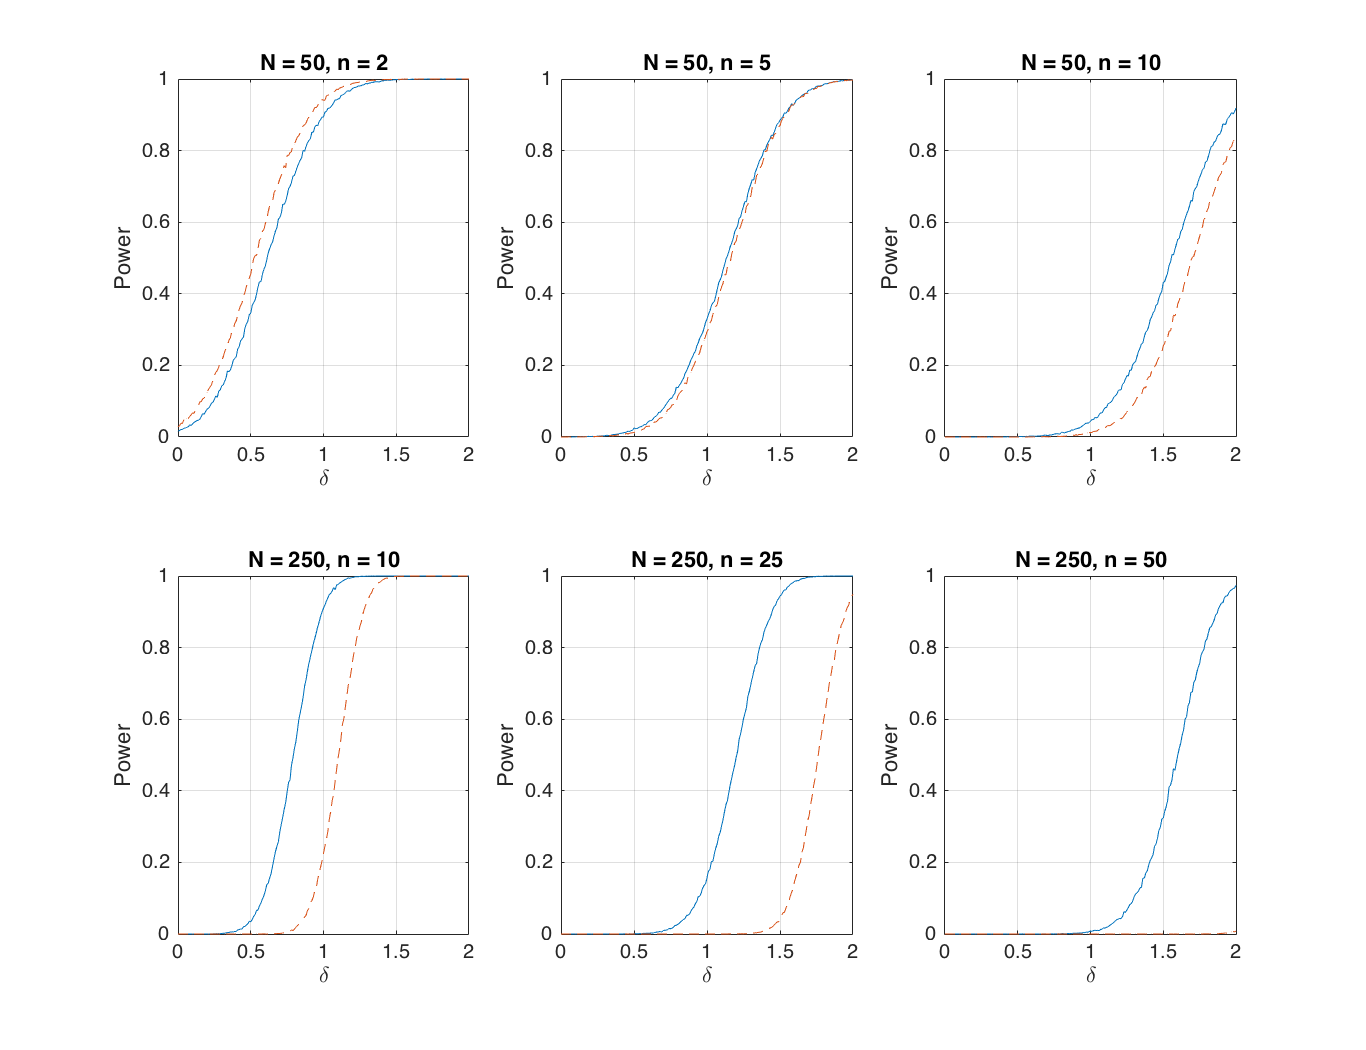
\includegraphics[width = \textwidth]{plotMultinomialPower}
\end{center}
\caption{Power curves as a function of $\delta$. The plots in the first row all have $m = 50$ and the second row $m = 250$. The solid line and the dashed line are the power for the selective test and Gupta and Nagel's test, respectively.}
\label{fig:power}
\end{figure}

\section{By How Much?}
\label{sec:confbound}

We can take the idea above further and construct confidence bound for $\theta_{[1]} - \max_{j \ne [1]} \theta_{j}$. This can be achieved by considering a statistical test, to see if $\theta_{[1]} - \max_{j \ne [1]} \theta_{j} \le \delta$, followed by the duality of confidence interval and statistical test.

Here we provide a more powerful Procedure 2' first. The confidence lower bound can be taken as the smallest $\delta$ such that we can reject $H_{0[1]}^\delta: \theta_{[1]} - \max_{j \ne [1]} \theta_{[j]} > \delta$. Once again this can be written as a union of null hypothesis
$$H_{0[1]}^\delta = \bigcup_{j \ne [1]} H_{0[1]j}: \theta_1 - \theta_j > \delta.$$
By \Cref{lma:union}, we can construct selective exact one-tailed $p$-values $p_{[1]j}$ for each of these by conditioning on $A_{[1]}$, $M_{[1]j}$ and $X_{\setminus\left\{[1], j\right\}}$, giving us an exact test for $H_{0[1]}$ by rejecting whenever $\max_{j \ne [1]} p_{[1]j} < \alpha$.

\begin{theorem}
The $p$-values constructed above satisfies $p_{[1][2]} \ge p_{[1]j}$ for any $j \ne [1]$.
\end{theorem}

\begin{proof}
Again we start with assuming $X_1 \ge \cdots \ge X_n$. The $p$-values in question are derived from the conditional law
$$\mathcal{L}_{\theta_1 - \theta_j = \delta} \left(D_{1j} \middle| D_{1j}, X_2, \ldots, X_n, A\right),$$
which is the truncated distribution
\begin{align*}
D_{1j} & \sim \exp\left(\left(\theta_1 - \theta_j\right) D_{1j} + \theta_2 X_2 + \cdots + \left(\theta_1 + \theta_j\right) M_{1j} + \cdots + \theta_n X_n \right) \\
& ~~~~~~~~ g\left(M_{1j} + D_{1j}, X_2, \ldots, M_{1j} - D_{1j}, \ldots X_n\right) 1_{A_1} \\
& \sim \exp\left(\delta D_{1j}\right) g\left(M_{1j} + D_{1j}, X_2, \ldots, M_{1j} - D_{1j}, \ldots X_n\right) 1_{A_1}.
\end{align*}

The $p$-values thus are
$$p_{1j} = \frac{\int_{D_{1j}}^\infty \exp\left(\delta z\right) g\left(M_{1j} + z, X_2, \ldots, M_{1j} - z, \ldots, X_n\right) \,dz}{\int_{\max\left\{X_2 - M_{1j}, 0\right\}}^\infty \exp\left(\delta z\right) g\left(M_{1j} + z, X_2, \ldots, M_{1j} - z, \ldots, X_n\right) \,dz}.$$

As before in \Cref{thm:seltest}, without loss of generality we assume $n = 3$. Once again it is sufficient to show that $p_{12} \ge p_{13}$. We have the same two cases. If $X_2 < M_{13}$, then
\begin{align*}
p_{12} & = \frac{\int_0^\infty \exp\left(\delta \left(z + D_{12}\right)\right) g\left(X_1 + z, X_2 - z, X_3\right) \,dz}{\int_{-D_{12}}^\infty \exp\left(\delta \left(z + D_{12}\right)\right) g\left(X_1 + z, X_2 - z, X_3\right) \,dz} \\
& = \frac{\int_0^\infty \exp\left(\delta z\right) g\left(X_1 + z, X_2 - z, X_3\right) \,dz}{\int_{-D_{12}}^\infty \exp\left(\delta z\right) g\left(X_1 + z, X_2 - z, X_3\right) \,dz} \\
p_{13} & = \frac{\int_0^\infty \exp\left(\delta \left(z + D_{13}\right)\right) g\left(X_1 + z, X_2, X_3 - z\right) \,dz}{\int_{-D_{13}}^\infty \exp\left(\delta \left(z + D_{13}\right)\right) g\left(X_1 + z, X_2, X_3 - z\right) \,dz} \\
& = \frac{\int_0^\infty \exp\left(\delta z\right) g\left(X_1 + z, X_2, X_3 - z\right) \,dz}{\int_{-D_{13}}^\infty \exp\left(\delta z\right) g\left(X_1 + z, X_2, X_3 - z\right) \,dz}
\end{align*}

The same argument in \Cref{fig:compare_rays} shows that $p_{12} \ge p_{13}$. This is again true for the case where $X_2 \ge M_{13}$ as well.
\end{proof}

In other words, Procedure 2' can be summarized as: Find the minimum $\delta$ such that $p_{12} \le \alpha$. And by construction, Procedure 2' gives exact $1-\alpha$ confidence bound for $\theta_{[1]} - \max_{j \ne [1]} \theta_j$.

\begin{corollary}
Assume the model~\eqref{eqn:expfam} holds and $g\left(x\right)$ is a Schur-concave function. Procedure 2 (the lower bound of unadjusted pairwise confidence interval) gives a conservative $1-\alpha$ lower confidence bound for $\theta_{[1]} - \max_{j \ne [1]} \theta_j$.
\end{corollary}

\begin{proof}
If the confidence bound $\delta^*$ is negative, we report $-\infty$ so it definitely is valid and conservative. On the other hand, if $\delta^* \ne 0$, then at $\delta^*$ the $p$-value $p_{12} = \alpha$. The denominator is the positive part of a positively skewed distribution, and thus bigger than half of the distribution. So the unadjusted pairwise test $p$-value from Procedure 2 comparing $X_1$ and $X_2$ is larger than $p_{12}$ from Procedure 2', rendering Procedure 2 conservative.
\end{proof}

Note that Procedure 2 reporting $-\infty$ in case of $\delta^*$ is rather extreme. In reality, we can always just adopt Procedure 2' in the case when Procedure 1 rejects. In fact, by Procedure 2', the multinomial example for polling in \Cref{sec:iowa} can give a stronger lower confidence bound, that $\log \pi_{\text{Trump}} - \max_{j \ne \text{Trump}} \log \pi_{j} \ge 0.103142$.

\section{Is the Runner-Up Really the Second Best, etc.?}
\label{sec:stepdown}

If one is interested in verifying more than just the ``winner'', this selective test can also be extended to a step-down procedure that verifies the ``first runner-up'' and ``second runner-up'' etc., while controlling the FWER.

Formally, we wish to find the biggest $j$ such that we can infer
$$\theta_{[1]} > \ldots > \theta_{[j]} > \max_{k>j} \theta_{[k]}.$$
If $j_0$ is the true value of $j$, the FWER refers to $\PP\left(j \ne j_0\right)$.

\begin{theorem}
There is a step-down procedure, which we will denote as Procedure 3', that infers $j_0$ above with the FWER controlled at $\alpha$.
\end{theorem}

\begin{proof}

This can be fitted into the selective sequential model selection framework proposed by \citet{Fithian:2015uj}. Given the observations $X_1 \ge \cdots \ge X_n$, drawn from an unknown distribution $F$, we consider the sequence of null hypothesis of
$$H_{0j}: \theta_j \le \max_{k > j} \theta_k.$$
Alternatively, we can think of them as a sequence of nested model
$$M_0\left(X\right) \subseteq M_1\left(X\right) \subseteq \cdots \subseteq M_n\left(X\right), ~~~~~~~~ M_j\left(X\right)^c = \left\{\theta_1 > \cdots > \theta_j > \max_{k > j} \theta_k\right\},$$
and the each $M_j$ depends on $X$ through the order of $X$. The step-down procedure for rejecting $H_{0j}$ is equivalent to selecting the smallest $j$ for which $F \in M_j\left(X\right)$.

We can construct selective $p$-values by conditioning on $M_j\left(X\right)$, as well as other nuisance parameters. Specifically, we are conditioning on the selection of the model $M_j\left(X\right)$. We can take $p_j$ to be the survival function of the conditional law
\begin{align}
&~ \mathcal{L}_{\theta_j = \theta_{j+1}} \left(D_{j\left(j+1\right)} \middle| M_j\left(X\right), X_1, \ldots, X_{j-1}, M_{j\left(j+1\right)}, X_{j+2}, \ldots, X_n\right) \nonumber \\
= &~ \mathcal{L}_{\theta_j = \theta_{j+1}} \left(D_{j\left(j+1\right)} \middle| \left\{X_1 > \ldots > X_j > \max_{k > j} X_k\right\}, X_1, \ldots, X_{j-1}, M_{j\left(j+1\right)}, X_{j+2}, \ldots, X_n\right) \nonumber \\
= &~ \mathcal{L}_{\theta_j = \theta_{j+1}} \left(D_{j\left(j+1\right)} \middle| \left\{X_{j-1} > X_j > M_{j\left(j+1\right)}\right\}, X_1, \ldots, X_{j-1}, M_{j\left(j+1\right)}, X_{j+2}, \ldots, X_n\right). \label{eqn:step_down_law}
\end{align}

\begin{figure}[htbp]
\begin{center}
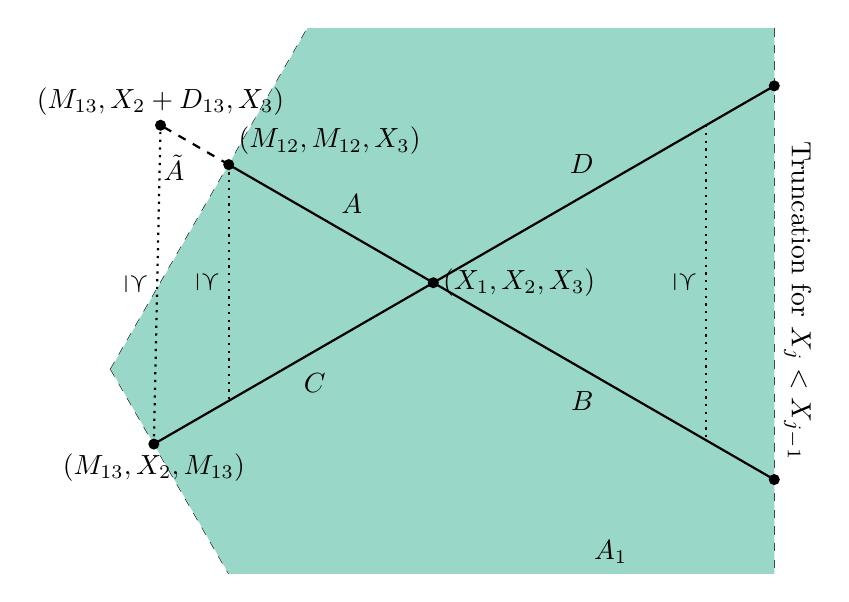
\begin{tikzpicture}
	\coordinate (C1) at (60:5);
	\coordinate (C2) at (300:3);
	\coordinate (A) at (60:3);
	\coordinate (B) at ($(A) + (330:3)$);
	\coordinate (C) at ($(0, 0)!(B)!(C2)$);
	\coordinate (D) at ($(A) + (150:1)$);
	\coordinate (C3) at ($(B) + (330:5)$);
	\coordinate (C4) at ($(B) + (30:5)$);
	\coordinate (C5) at ($(C3)!(C1)!(C4)$);
	\coordinate (C6) at ($(C3)!(C2)!(C4)$);
	\draw[dashed] (0, 0) -- (C1);
	\draw[dashed] (0, 0) -- (C2);
	\draw[dashed] (C5) -- (C6) node[midway, above, rotate = -90] {Truncation for $X_j < X_{j-1}$};
	\fill[mid_green] (0, 0) -- (C1) -- (C5) -- (C6) -- (C2) -- cycle;
	\node[above] at ($(C2)!0.7!(C6)$) {$A_1$};
	\draw[thick] (A) -- (B) node[midway, above right] {$A$};
	\draw[thick] (B) -- (C3) node[midway, below left] {$B$};
	\fill (C3) circle(2pt);
	\fill (A) circle(2pt) node[above right] {$\left(M_{12}, M_{12}, X_3\right)$};
	\fill (B) circle(2pt) node[right] {$\left(X_1, X_2, X_3\right)$};
	\draw[thick] (C) -- (B) node[midway, below right] {$C$};
	\node[below] at (C) {$\left(M_{13}, X_2, M_{13}\right)$};
	\draw[thick] (B) -- (C4) node[midway, above left] {$D$};
	\fill (C4) circle(2pt);
	\fill ($(0, 0)!(B)!(C2)$) circle(2pt);
	\draw[thick, dashed] (A) -- (D) node[midway, below left] {$\tilde{A}$};
	\fill (D) circle(2pt) node[above] {$\left(M_{13}, X_2 + D_{13}, X_3\right)$};
	\draw[thick, dotted] (C) -- (D) node[midway, below, rotate=-90] {$\succeq$};
	\draw[thick, dotted] (A) -- ++(0, -3) node[midway, below, rotate=-90] {$\succeq$};
	\draw[thick, dotted] ($(B) + (30:4)$) -- ($(B) + (330:4)$) node[midway, below, rotate=-90] {$\succeq$};
\end{tikzpicture}
\end{center}
\caption{The two $p$-values constructed corresponds to taking integrals of $g$ along these segments, that lie on a level set of $x_j + x_{j+1} + x_k$. The dashed line corresponds to extension in \Cref{eqn:int_extension}. The dotted line on the far right is the truncation that enforces $X_j < X_{j-1}$.}
\label{fig:crop_rays}
\end{figure}

Here we are only comparing $X_j$ to $X_{j+1}$ by \Cref{sec:winnerbest}. The upper truncation for $X_j$ can be represented by cropping \Cref{fig:compare_rays} along a vertical line, shown in \Cref{fig:crop_rays}, thus the proof of \Cref{thm:seltest} on sufficiency to compare $X_1$ and $X_2$ remains valid with appropriate conditioning. Again we can construct the $p$-values as in \Cref{eqn:p1j} for $k>j$.

$$p_{jk} = \frac{\int_{D_{jk}}^{X_{j-1}} g\left(X_1, \ldots, M_{jk} + z, \ldots, M_{jk} - z, \ldots, X_n\right) \,dz}{\int_{\max\left\{X_{j+1} - M_{jk}, 0\right\}}^{X_{j-1}} g\left(X_1, \ldots, M_{jk} + z, \ldots, M_{jk} - z, \ldots, X_n\right) \,dz}.$$

Hence similar to the proof of \Cref{thm:seltest}, Schur-concavity ensures $p_{j\left(j+1\right)} \ge p_{jk}$ for all $k>j$, meaning that it is sufficient to compare $X_j$ and $X_{j+1}$. In fact, we can take $p_j = p_{j\left(j+1\right)}$. These are valid selective $p$-value as required in \citet{Fithian:2015uj}, as
$$\PP_F \left(p_j \le \alpha \middle| M_{j-1}\left(X\right)\right) \le \alpha \text{ a.s.}, ~~~~~~~~ F \in M_{j-1}\left(X\right)$$
by tower property.

The conditioning above indeed holds some significance. The sufficient filtration \citep{Fithian:2015uj} $\mathscr{F}_k$ is given as the $\sigma$-field
\begin{align*}
\mathscr{F}_k & = \sigma\left(M_0\left(X\right), \ldots, M_j\left(X\right), X_1, \ldots, X_{j-1}, \frac{X_j + X_{j+1}}{2}, X_{j+2}, \ldots, X_n\right) \\
& = \sigma\left(\left\{X_1 > \ldots > X_j > \max_{k>j} X_k\right\}, X_1, \ldots, X_{j-1}, \frac{X_j + X_{j+1}}{2}, X_{j+2}, \ldots, X_n\right) \\
& = \sigma\left(M_j\left(X\right), X_1, \ldots, X_{j-1}, \frac{X_j + X_{j+1}}{2}, X_{j+2}, \ldots, X_n\right),
\end{align*}
which is the conditioning we used just now. Hence the nested sequence of model satisfies the subpath sufficiency principle, and the $p$-values sequence $p_j$ is independent on nulls, as defined in and shown in Theorem 4 of \citet{Fithian:2015uj}. Thus the step-down procedure where we keep rejecting $H_{0j}$ until the first time that $p_j > \alpha$ controls FWER.
\end{proof}

\begin{corollary}
Assume the model~\eqref{eqn:expfam} holds and $g\left(x\right)$ is a Schur-concave function. Procedure 3 is a conservative step-down procedure with FWER no larger than $\alpha$.
\end{corollary}

\begin{proof}
The $p$-values $p_{j\left(j+1\right)}$ obtained in Procedure 3' are always smaller than their counterpart in Procedure 3, as the upper truncation at $X_{j-1}$ is on the upper tail. Therefore Procedure 3 is conservative and definitely valid.
\end{proof}

\section{Discussion}
\label{sec:disc}

Our selective test procedure allows us to untangle multiple comparisons based on correlated observations easily, while avoiding the pitfalls of selective inference. To illustrate, we look at a past psychology study done by \citet{Uhls:2012gf}.

\begin{table}[htbp]
\begin{center}
\begin{tabular}{c c}
	\hline
	Value & Count \\
	\hline
	Achievement & $3$ \\
	Benevolence & $5$ \\
	Fame & $8$ \\
	Community feeling & $2$ \\
	Financial success & $1$ \\
	Self-acceptance & $0$ \\
	Image & $0$ \\
	Other & $1$ \\
	\hline
\end{tabular}
\end{center}
\caption{The number of study participants who chose each value as their top desired one. Since only one options can be chosen, these observations are inherently multinomial.}
\label{tbl:fame}
\end{table}

A sample of $20$ students from elementary and middle schools were asked to choose a top ``value'' from 7 different options: achievement, benevolence, fame, community feeling, financial success, self-acceptance, image and other. The results are tabulated in \Cref{tbl:fame}. The study postulates that fame is significantly the top value of choice. It proceeds to perform a binomial test for the null hypothesis that the participants chose among the $7$ options uniformly and concluded with a $p$-value of $0.006$ that fame is indeed the top desired value. The analysis failed to address the ``winner's curse'', as well as the intricate dependence among the observations. Our paper addressed these two issues and provided a simple test --- perform a unadjusted (two-tailed) binomial test of the winner and the runner-up. In this case, we test if $8$ is a significant observation in $\text{Binomial}\left(8 + 5, 0.5\right)$. The two-tailed $p$-value is $0.580811$, suggesting that the study was inconclusive.

\bibliographystyle{plainnat}
\bibliography{papers,additional}

\end{document}